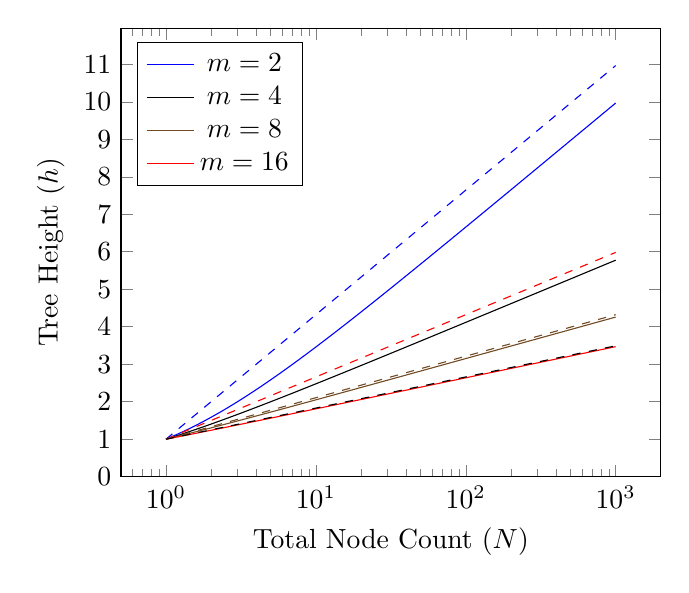
\begin{tikzpicture}
	\begin{axis}
		[
			xlabel={Total Node Count ($N$)},
			ylabel={Tree Height ($h$)},
			domain=1:1000,
			xmode=log,
			ytick distance=1,
			legend pos=north west,
			smooth
		]
		\pgfplotsinvokeforeach{2,4,8,16} {
			\addplot+[cycle list name=color list, mark=none]
				{ln(1 - x*(1-#1)) / ln(#1)};
			\addlegendentry{$m=#1$}
		}
		\pgfplotsset{cycle list shift=-4}
		\pgfplotsinvokeforeach{2,4,8,16} {
			\addplot+[cycle list name=color list, mark=none, dashed]
				{1+ln(x)/ln(#1)};
		}
	\end{axis}
\end{tikzpicture}
